% \end{center}

% sdasasasas \\
% \begin{adjustwidth}{-1cm}{-1cm}% adjust the L and R margins by 1 inch
%   test
% \end{adjustwidth}


% & Streaming unterwegs & Einfache Webcam-Streams & Reproduzierbare Livestreams, die eine einmalige Einrichtung erfordern & Livestream-Einrichtung mit vielen Anpassungsmöglichkeiten \\ \hline
%
% & Schnell und einfach & Schnell und einfach & Produziert & Tent-Poling-Video \\ \hline
% & Gering & Gering & Mittel/Hoch & Hoch \\ \hline
% & Mobiltelefon mit Kamera & Computer mit Webcam & Computer mit Webcam und Streamingsoftware & Computer Kamera Streamingsoftware \\ \hline
%   & Livestream in wenigen Schritten über ein Handy starteb & Livestream mit wenigen Klicks starten & Eine Liveadresse für wiederholbare Livestreams & Eine benutzerdefinierte Live-veranstaltung erstellen, welche auch ein Multicamstream sein kann. \\ \hline



% \newlength{\breite}
% \breite25mm
% \begin{tabular}{|p{\breite}|p{\breite}|p{\breite}|p{\breite}|}
% \hline
% \multicolumn{2}{|l|}{Feld über zwei Spalten}feld&Feld&Feld\\
% \hline
% Feld&Feld&\multicolumn{2}{|l|}{Feld über zwei Spalten}\\
% \hline
% %Feld&\multirow{2}{3cm}{Feld über zwei Zeilen}&Feld\\
% Feld&\multirow{2}{\breite}{Feld über zwei Zeilen}&\multicolumn{2}{|p{3cm}|}{\multirow{2}{5cm}{Feld über zwei Zeilen und zwei Spalten}}\\
% \cline{0-0}
% Feld&&\multicolumn{2}{|c|}{}\\
% \hline
% \end{tabular}

% \begin{table}[htb]
%       \begin{tabular*}{\linewidth}{@{\extracolsep{\fill}}*8l@{}} \toprule
%       Spalte1 & Spalte2 & Spalte3 & Spalte4 & Spalte5 & Spalte6 & Spalte7 & Spalte8 \\ \midrule
%       AA      & BB      & CC      & DD      & EE      & FF      & GG      & HH      \\
%       AA      & BB      & CC      & DD      & EE      & FF      & GG      & HH      \\ \bottomrule
%     \end{tabular*}
% \end{table}

\sect{Vorbereitung des Streams}

Bei einem Livestream gibt es einiges bezüglich des Chats zu beachten:
\begin{itemize}
  \item Moderatoren sollten vor einem Chat zugewiesen sein.
  \item Blockieren von unangemessenen Wörtern oder Links aktivieren.
  \item Langsamen Modus aktivieren damit Zuschauer nicht den Chat zuspammen können.
  \item \grqq{}Zur Überprüfung zurückhalten\grqq{} aktivieren damit problematische Wörter nicht im chat erscheinen.
\end{itemize}

\sect{Geplante Veröffentlichungen}


\sect{Während des Streams}
\sect{Voting}
\sect{Fazit}


% 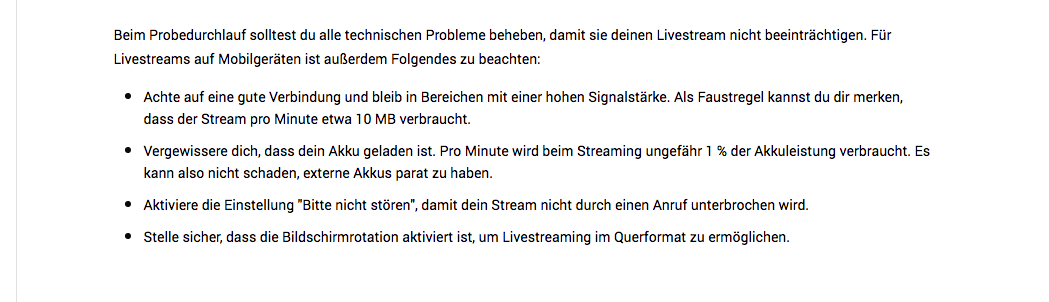
\includegraphics[scale=0.5]{./pictures/vordemstream.png}
%
% 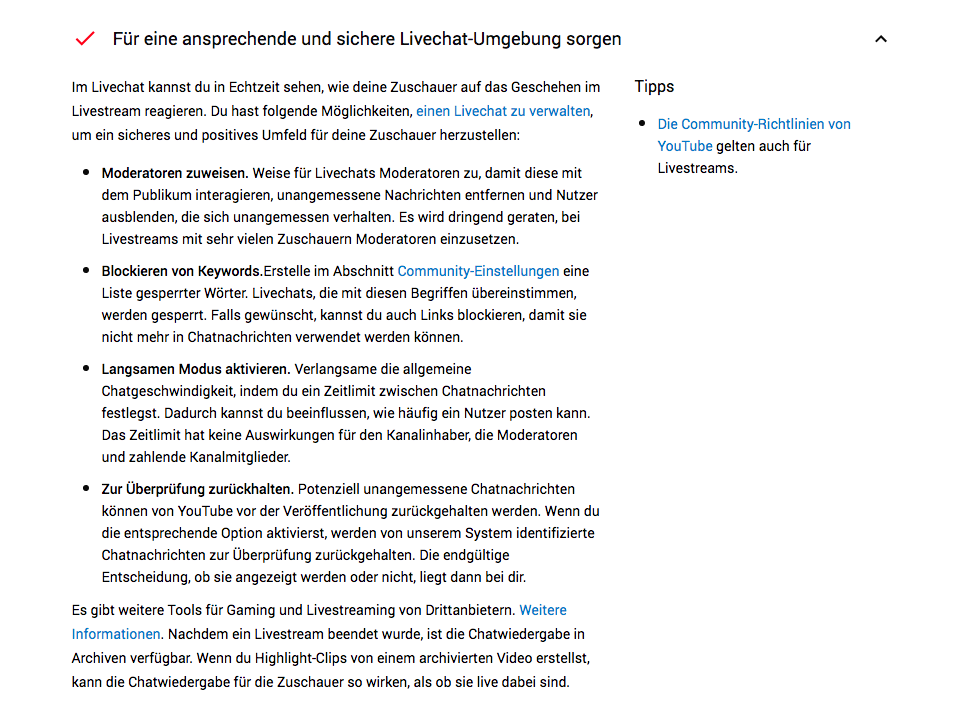
\includegraphics[scale=0.5]{./pictures/livechat.png}

% 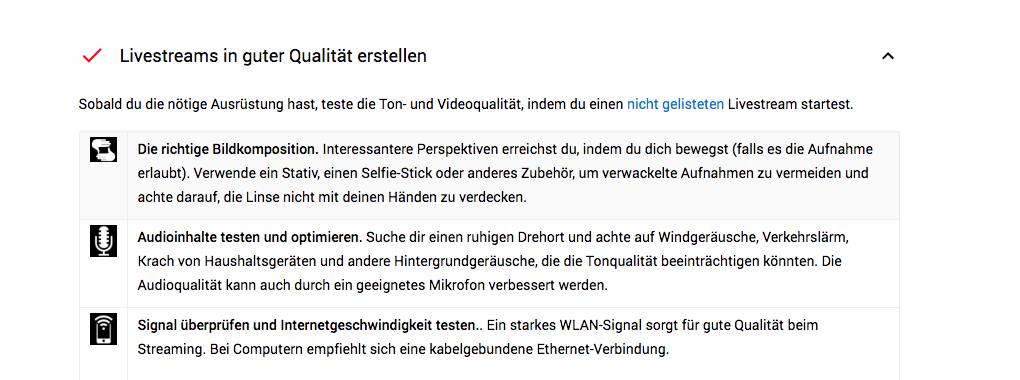
\includegraphics[scale=0.5]{./pictures/preflightchecks.png}
% 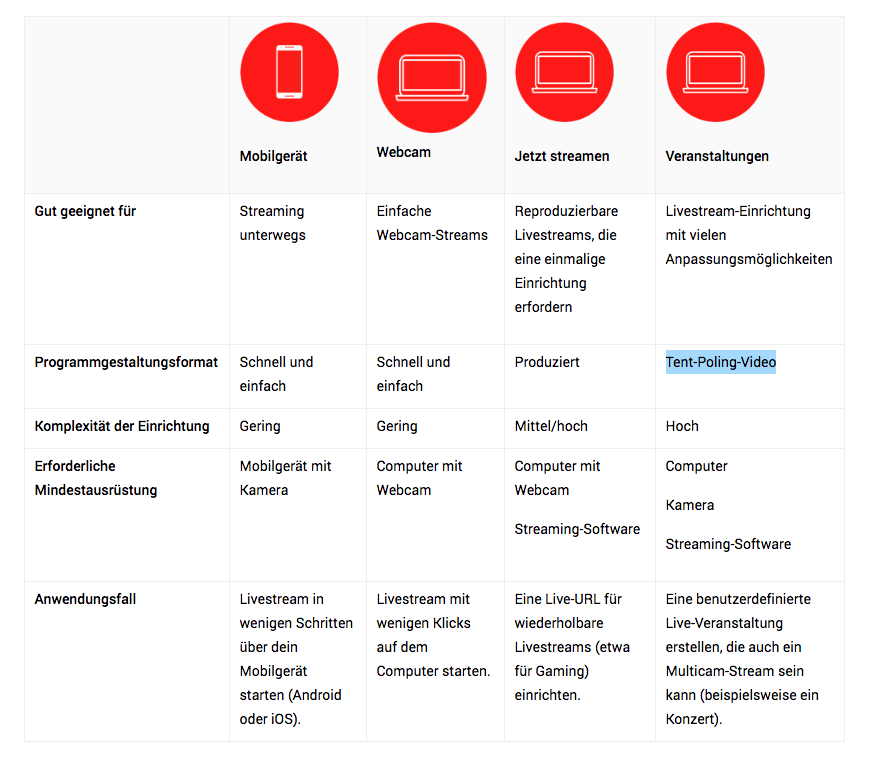
\includegraphics[scale=0.5]{./pictures/streamingarten.png}
%
%
%















%
% \begin{tabular}{ll}
% \centering
% \glqq Text\grqq{} und \flqq Text\frqq  & \verb+ \glqq Text\grqq{} und \flqq Text\frqq+\\
% \glq Text\grq{} und \flq Text\frq  & \verb+ \glq Text\grq{} und \flq Text\frq+
% \end{tabular}





% \definecolor{fulda_green}{rgb}{.38,.74,.10}
% \definecolor{fulda_lightgreen}{rgb}{.64,.85,.40}
% \definecolor{fulda_lightgray}{gray}{.4}
% \definecolor{fulda_subtitle}{rgb}{.38,.74,.10}
% \definecolor{fulda_title}{gray}{.0}
% \definecolor{fulda_chapter}{rgb}{.38,.74,.10}
% \definecolor{fulda_section}{rgb}{.38,.74,.10}
% \definecolor{fulda_subsection}{gray}{.4}
% \definecolor{fulda_part}{gray}{1}
% \definecolor{fulda_partnumber}{rgb}{.79,1,.55}
% \definecolor{fulda_partback}{rgb}{.64,.85,.40}
% \definecolor{fulda_highlighttitle}{rgb}{.38,.74,.10}
% \definecolor{fulda_highlightbody}{rgb}{.79,1,.55}
% \definecolor{fulda_highlighttitletext}{gray}{1}
% \definecolor{lightgray}{rgb}{0.93,0.95,1.0}
% \definecolor{darkgreen}{RGB}{82,130,179}
